%% ACM Small Standard Format (without copyright/journal info)
\documentclass[acmsmall,screen,nonacm]{acmart}

%% Remove ACM reference format
\settopmatter{printacmref=false, printccs=false}

%% Essential packages
\usepackage{booktabs}
\usepackage{amsfonts}
\usepackage{mathtools}
\usepackage{threeparttable}

%% Title and author information
\title{Assignment 2: Analysis of Probabilistic Data Structures}

\author{Riley Eaton}
\affiliation{%
  \institution{University of British Columbia}
  \city{Kelowna}
  \state{BC}
  \country{Canada}
}

\begin{document}

\maketitle

\section{Introduction} \label{sec:introduction}
Probabilistic data structures sacrifice perfect accuracy for significant gains in space efficiency and computational speed. Unlike exact data structures that provide deterministic guarantees, probabilistic data structures allow controlled error rates in exchange for using substantially less memory and faster query times. This trade-off makes them invaluable for processing massive datasets where storing complete information is impractical.

This report analyzes three fundamental probabilistic data structures---Bloom filters, Count-Min sketches, and LogLog---each designed to solve a distinct problem in data stream processing and large-scale data analysis.

\subsection{Bloom Filter}

The Bloom filter, introduced by Burton Bloom in 1970~\cite{bloom1970space}, is a space-efficient probabilistic data structure for testing set membership. Given an element, a Bloom filter answers the query ``Is this element in the set?'' with two possible responses: ``definitely not in the set'' or ``possibly in the set.'' False positives are possible, but false negatives are not.

The structure consists of a bit array of size $m$ and $k$ independent hash functions. When inserting an element, each hash function maps the element to a position in the bit array, and those positions are set to 1. To query an element, the same hash functions are applied; if all corresponding positions are 1, the filter returns ``possibly in set,'' otherwise ``definitely not in set.''

Bloom filters have found widespread application in network systems~\cite{broder2004network}, including web caching (to avoid caching one-hit wonders), distributed databases (to reduce disk lookups), and content delivery networks. Modern systems like Google Chrome use Bloom filters to check URLs against malicious site databases without storing the entire list locally.

The main trade-off is the false positive rate, which can be controlled by adjusting $m$ (bit array size) and $k$ (number of hash functions). The false positive probability decreases exponentially with the amount of memory allocated, making Bloom filters extremely space-efficient for applications that can tolerate occasional false positives.

\subsection{Count-Min Sketch}

The Count-Min sketch, developed by Cormode and Muthukrishnan in 2005~\cite{cormode2005improved}, extends the concept of probabilistic data structures to frequency estimation in data streams. Rather than simply testing membership, it estimates how many times each element has appeared in a stream.

The data structure uses a two-dimensional array of counters with width $w$ and depth $d$. When an element arrives, hash functions map it to positions that are incremented. To estimate frequency, the sketch returns the minimum value across all positions, providing an upper bound on the true frequency.

Count-Min sketches are crucial for many streaming applications: finding heavy hitters in network traffic, tracking popular queries in search engines, detecting DDoS attacks, and analyzing social media trends. The sketch guarantees that frequency estimates are never underestimated but may be overestimated due to hash collisions.

The accuracy is controlled by two parameters: $\epsilon$ (the error bound) and $\delta$ (the failure probability). By choosing $w = \lceil e/\epsilon \rceil$ and $d = \lceil \ln(1/\delta) \rceil$, the sketch ensures that with probability at least $1-\delta$, the error in any frequency estimate is at most $\epsilon N$, where $N$ is the total number of items processed.

\subsection{LogLog}

The LogLog algorithm, introduced by Durand and Flajolet in 2003~\cite{durand2003loglog}, addresses the cardinality estimation problem: determining the number of distinct elements in a large multiset or data stream. This is a fundamental problem in database query optimization, network monitoring, and data analytics.

The algorithm uses properties of hash functions and probabilistic counting. It hashes each element and examines the binary representation, specifically the position of the first 1-bit. Elements with long runs of leading zeros indicate large cardinality.

To improve accuracy, LogLog partitions the input stream into $m = 2^b$ substreams using the first $b$ bits of each hash value. Each substream maintains its own maximum leading-zero count. The final cardinality estimate is computed as the harmonic mean of the estimates from all substreams, multiplied by a correction factor.

LogLog performs cardinality estimation using only $m$ small registers (each storing $\log_2 \log_2 n_{\text{max}}$ bits, where $n_{\text{max}}$ is the maximum expected cardinality). This logarithmic-logarithmic space requirement is the origin of the algorithm's name. The standard error is approximately $1.30/\sqrt{m}$, meaning accuracy improves with the square root of the number of registers.

Applications include database query optimization (estimating the size of joins), web analytics (counting unique visitors), and distributed systems (tracking distinct items across multiple nodes). Later variants like HyperLogLog further improved the accuracy and are now widely deployed in systems like Redis and Google BigQuery.


\section{Computational Complexity} \label{sec:complexity}
The efficiency of probabilistic data structures makes them valuable for large-scale applications. This section analyzes the time and space complexity of Bloom filters, Count-Min sketches, and LogLog algorithms, explaining the parameters that govern their performance.

\subsection{Bloom Filter Complexity}

\subsubsection{Space Complexity}

A Bloom filter uses a bit array of size $m$ bits, giving a space complexity of $O(m)$. The optimal size depends on the expected number of elements $n$ and desired false positive rate $p$:

\begin{equation}
m = -\frac{n \ln p}{(\ln 2)^2} \approx -1.44 n \log_2 p
\end{equation}

For example, to store 1 million elements with a 1\% false positive rate requires approximately 9.6 bits per element, totaling about 1.2 MB---far less than storing the elements themselves.

The number of hash functions $k$ that minimizes the false positive rate is:

\begin{equation}
k = \frac{m}{n} \ln 2 \approx 0.693 \frac{m}{n}
\end{equation}

Each bit in the filter stores a single bit of information, making Bloom filters extremely space-efficient compared to hash tables or sets that must store complete element representations.

\subsubsection{Time Complexity}

Both insertion and query operations require computing $k$ hash functions and accessing $k$ positions in the bit array, yielding:

\begin{itemize}
    \item \textbf{Insertion}: $O(k)$ time
    \item \textbf{Query}: $O(k)$ time
\end{itemize}

Since $k$ is typically a small constant (often 3--10 for practical false positive rates), these operations are effectively constant time $O(1)$ in practice~\cite{bloom1970space}.

\subsection{Count-Min Sketch Complexity}

\subsubsection{Space Complexity}

A Count-Min sketch maintains a two-dimensional array of counters with width $w$ and depth $d$. Each counter typically uses a fixed number of bits (e.g., 32 or 64 bits). The space complexity is:

\begin{equation}
O(w \cdot d) = O\left(\frac{e}{\epsilon} \cdot \ln \frac{1}{\delta}\right)
\end{equation}

where:
\begin{itemize}
    \item $\epsilon$ is the error bound (additive error in frequency estimates)
    \item $\delta$ is the failure probability
    \item $e \approx 2.718$ is Euler's number
\end{itemize}

The dimensions are chosen as $w = \lceil e/\epsilon \rceil$ and $d = \lceil \ln(1/\delta) \rceil$ to achieve the desired accuracy guarantees~\cite{cormode2005improved}.

For example, with $\epsilon = 0.01$ (1\% error) and $\delta = 0.01$ (99\% confidence), the sketch requires $w \approx 272$ and $d \approx 5$, totaling 1,360 counters. Using 32-bit counters, this consumes approximately 5.3 KB regardless of stream size.

\subsubsection{Time Complexity}

Update and query operations both hash the element with $d$ hash functions and access $d$ counters:

\begin{itemize}
    \item \textbf{Update}: $O(d) = O(\ln(1/\delta))$ time
    \item \textbf{Query}: $O(d) = O(\ln(1/\delta))$ time
\end{itemize}

With typical values of $d$ (3--10), these operations are constant time in practice. Importantly, the time complexity is independent of the stream length and the number of distinct elements.

\subsection{LogLog Complexity}

\subsubsection{Space Complexity}

LogLog uses $m = 2^b$ registers, where each register stores the maximum number of leading zeros observed in its substream. For a maximum expected cardinality of $n_{\max}$, each register requires:

\begin{equation}
\log_2 \log_2 n_{\max} \text{ bits}
\end{equation}

The total space complexity is:

\begin{equation}
O(m \log \log n_{\max})
\end{equation}

This doubly-logarithmic dependence on $n_{\max}$ is notable. For example, to estimate cardinalities up to $2^{32} \approx 4.3$ billion using $m = 1024$ registers, each register needs only 5 bits, totaling 640 bytes. Even for datasets with trillions of elements ($n_{\max} = 2^{64}$), each register requires only 6 bits~\cite{durand2003loglog}.

The standard error of the estimate is:

\begin{equation}
\sigma \approx \frac{1.30}{\sqrt{m}}
\end{equation}

Thus, quadrupling the number of registers (and the memory usage) halves the standard error.

\subsubsection{Time Complexity}

Processing each element involves:
\begin{enumerate}
    \item Computing a hash function: $O(1)$ amortized time
    \item Extracting the first $b$ bits to determine the register: $O(1)$ time
    \item Counting leading zeros: $O(1)$ time (bounded by hash output size)
    \item Updating one register: $O(1)$ time
\end{enumerate}

Therefore:
\begin{itemize}
    \item \textbf{Update}: $O(1)$ time per element
    \item \textbf{Cardinality estimation}: $O(m)$ time to aggregate all register values
\end{itemize}

The estimation step requires computing the harmonic mean across all $m$ registers, but this is typically done once after processing the entire stream.

\subsection{Comparative Analysis}

Table~\ref{tab:complexity_comparison} summarizes the time and space complexity of the three data structures.

\begin{table}[t]
\centering
\begin{tabular}{@{}llll@{}}
\toprule
\textbf{Data Structure} & \textbf{Space} & \textbf{Update} & \textbf{Query} \\
\midrule
Bloom Filter & $O(m)$ & $O(k)$ & $O(k)$ \\
 & $m = -\frac{n \ln p}{(\ln 2)^2}$ & $k = \frac{m}{n} \ln 2$ & $k = \frac{m}{n} \ln 2$ \\[0.5em]
Count-Min Sketch & $O(wd)$ & $O(d)$ & $O(d)$ \\
 & $w = \lceil e/\epsilon \rceil$ & $d = \lceil \ln(1/\delta) \rceil$ & $d = \lceil \ln(1/\delta) \rceil$ \\[0.5em]
LogLog & $O(m \log \log n_{\max})$ & $O(1)$ & $O(m)$\textsuperscript{*} \\
 & $m = 2^b$ registers & per element & for estimation \\
\bottomrule
\end{tabular}
\caption{Computational complexity comparison of the three probabilistic data structures. Parameters: $n$ (expected elements), $p$ (false positive rate), $\epsilon$ (error bound), $\delta$ (failure probability), $m$ (number of registers/bits), $k$ (hash functions), $w$ (width), $d$ (depth), $n_{\max}$ (maximum cardinality). \textsuperscript{*}LogLog estimation aggregates $m$ registers; updates are $O(1)$ per element.}
\label{tab:complexity_comparison}
\end{table}

All three structures achieve sublinear space complexity relative to storing complete element information. Bloom filters and Count-Min sketches provide constant-time operations for practical parameter choices, while LogLog offers the most aggressive space compression through its doubly-logarithmic dependence on the maximum cardinality. The choice among these structures depends on the specific problem: set membership (Bloom filter), frequency estimation (Count-Min sketch), or cardinality estimation (LogLog).


\section{Dataset} \label{sec:dataset}
A synthetic dataset modeled after web server access logs was generated to comprehensively evaluate the three probabilistic data structures. This dataset type was chosen because it naturally supports testing all three data structures while reflecting realistic usage patterns.

\subsection{Dataset Design}

The synthetic dataset simulates web server traffic with the following attributes:

\begin{itemize}
    \item \textbf{User IDs}: Represented as IP addresses, serving as identifiers for unique visitors
    \item \textbf{URLs}: Endpoint paths accessed by users (e.g., \texttt{/home}, \texttt{/products})
    \item \textbf{Timestamps}: Sequential timestamps spanning the access log period
    \item \textbf{Request metadata}: HTTP method (GET, POST, etc.), status codes, and user agents
\end{itemize}

This design allows testing each data structure with its intended use case:

\begin{enumerate}
    \item \textbf{Bloom Filter}: Set membership testing for URLs (``Has this endpoint been accessed before?'')
    \item \textbf{Count-Min Sketch}: Frequency estimation for URLs (``How many times was each endpoint accessed?'')
    \item \textbf{LogLog}: Cardinality estimation for user IDs (``How many unique visitors were received?'')
\end{enumerate}

\subsection{Zipfian Distribution}

Real-world web traffic exhibits highly skewed access patterns where a small number of pages receive the majority of traffic~\cite{broder2004network,breslau1999web}. To capture this phenomenon, both user activity and URL popularity are modeled using a Zipfian (power-law) distribution~\cite{breslau1999web} with parameter $\alpha = 1.0$. Under this distribution, the probability of selecting the $k$-th ranked item is:

\begin{equation}
    P(k) = \frac{1/k^{\alpha}}{\sum_{i=1}^{N} 1/i^{\alpha}}
\end{equation}

where $N$ is the total number of unique items. This creates a realistic scenario where:

\begin{itemize}
    \item The most popular URL receives $\sim$13\% of all requests (133,012 out of 1,000,000 in the large dataset)
    \item The median URL receives only 37 requests
    \item Most users make few requests, while power users dominate traffic
\end{itemize}

This distribution is critical for testing probabilistic data structures because it represents the challenging real-world conditions under which these structures provide the most value---handling skewed data efficiently.

\subsection{Dataset Sizes}

Three dataset sizes were generated to evaluate scalability and accuracy trade-offs:

\begin{table}[h]
\centering
\begin{tabular}{@{}lrrr@{}}
\toprule
\textbf{Size} & \textbf{Events} & \textbf{Unique Users} & \textbf{Unique URLs} \\
\midrule
Small  & 10,000     & 906       & 100  \\
Medium & 100,000    & 8,556     & 500  \\
Large  & 1,000,000  & 47,382    & 1,000 \\
\bottomrule
\end{tabular}
\caption{Dataset sizes and characteristics. Unique counts reflect actual values observed after Zipfian sampling from larger pools (1,000, 10,000, and 50,000 users respectively). Note: The large dataset is not included in the GitHub repository due to file size limitations (103.68 MB exceeds GitHub's 100 MB limit) but can be regenerated using the provided generation script.}
\label{tab:dataset_sizes}
\end{table}

\subsection{Ground Truth and Validation}

Each dataset includes a ground truth file containing exact statistics computed during generation:

\begin{itemize}
    \item Actual unique counts (users and URLs)
    \item Exact frequency distributions for all items
    \item Top-10 most frequent users and URLs
    \item Distribution statistics (min, max, median frequencies)
\end{itemize}

This ground truth allows precise measurement of estimation errors for each probabilistic data structure. All datasets are generated with a fixed random seed (\texttt{seed=42}) to ensure reproducibility of experimental results.

\subsection{Data Format}

The dataset is provided in CSV format (complete logs), TXT streams (simplified testing), and JSON (ground truth statistics). The stream files provide simplified inputs for benchmarking individual data structure operations without parsing overhead.


\section{Experiments} \label{sec:experiments}
To empirically validate the theoretical complexity analysis and evaluate the practical performance of the implementations, a comprehensive benchmark suite was conducted measuring memory usage, throughput, and scalability characteristics. The experiments were designed to test each data structure under realistic workloads while maintaining comparability across structures.

\subsection{Experimental Setup}

\subsubsection{Implementation Details}

All three data structures were implemented from scratch using only Python's standard library, without external dependencies such as NumPy or specialized hashing libraries. This constraint ensures fair comparison and demonstrates the fundamental algorithms without optimization shortcuts. The implementations include:

\begin{itemize}
    \item \textbf{Bloom Filter}: Configured with $m = 1024$ bits and $k = 7$ hash functions, targeting approximately 1\% false positive rate
    \item \textbf{Count-Min Sketch}: Configured with $w = 272$ (width) and $d = 5$ (depth), corresponding to $\epsilon = 0.01$ and $\delta = 0.01$
    \item \textbf{LogLog}: Configured with $m = 1024$ registers ($b = 10$ bits), each storing up to 6 bits for leading zero counts
\end{itemize}

\subsubsection{Dataset Characteristics}

Synthetic datasets were generated following a Zipfian distribution with parameter $\alpha = 1.0$ (as described in Section~3), providing a realistic test of skewed access patterns.

\subsubsection{Benchmark Methodology}

Three categories of experiments were conducted:

\begin{enumerate}
    \item \textbf{Memory Efficiency}: Actual memory footprint was measured using Python's \texttt{sys.getsizeof()} on identical dataset sizes. This enables direct comparison across structures.

    \item \textbf{Insert Throughput}: Measured operations per second during bulk insertion, averaged over multiple runs to reduce variance

    \item \textbf{Scalability Analysis}: Tested performance across varying dataset sizes:
    \begin{itemize}
        \item Bloom Filter: 50, 125, 250, 375, 500 elements (smaller scale due to fixed bit array)
        \item Count-Min Sketch: 10K, 50K, 100K, 500K elements
        \item LogLog: 10K, 50K, 100K, 500K elements
    \end{itemize}
\end{enumerate}

The different scale ranges reflect the practical use cases for each structure: Bloom filters for moderate-sized sets with strict space constraints, while Count-Min sketches and LogLog target streaming applications with potentially unbounded data volumes.

Based on the complexity analysis in Section~2, LogLog is expected to show highest throughput ($O(1)$ updates), Bloom Filter to have lowest absolute memory (bit-level storage), and Count-Min Sketch to show best per-element efficiency at scale (fixed memory amortized over unbounded streams).

The benchmark results reveal both expected and surprising performance characteristics, validating some theoretical predictions while challenging others. This section presents the empirical measurements and analyzes discrepancies between theory and practice.

\subsection{Performance Summary}

Table~\ref{tab:performance_results} summarizes the measured performance metrics for all three data structures on comparable dataset configurations.

\begin{table}[h]
\centering
\begin{tabular}{@{}lccc@{}}
\toprule
\textbf{Data Structure} & \textbf{Memory (KB)} & \textbf{Insert Throughput (ops/sec)} & \textbf{Bytes per Element} \\
\midrule
Bloom Filter & 0.68 & 166,718 & 1.20\textsuperscript{\textdagger} \\
Count-Min Sketch & 5.41 & 85,420 & 0.0554 \\
LogLog & 16.10 & 170,714 & 1.93 \\
\bottomrule
\end{tabular}
\caption{Benchmark performance summary. All structures tested on Zipfian-distributed datasets. \textsuperscript{\textdagger}Bloom Filter bytes per element calculated from bits per element (9.586 bits / 8).}
\label{tab:performance_results}
\end{table}

\subsection{Comparative Analysis}

Figure~\ref{fig:memory_performance} presents side-by-side comparisons of memory usage and insertion throughput. The results confirm our memory usage predictions: Bloom Filter achieves the lowest absolute memory footprint (0.68 KB), followed by Count-Min Sketch (5.41 KB) and LogLog (16.10 KB). However, this ranking reverses when considering per-element efficiency at scale, as demonstrated in the scalability analysis.

\begin{figure}[h]
\centering
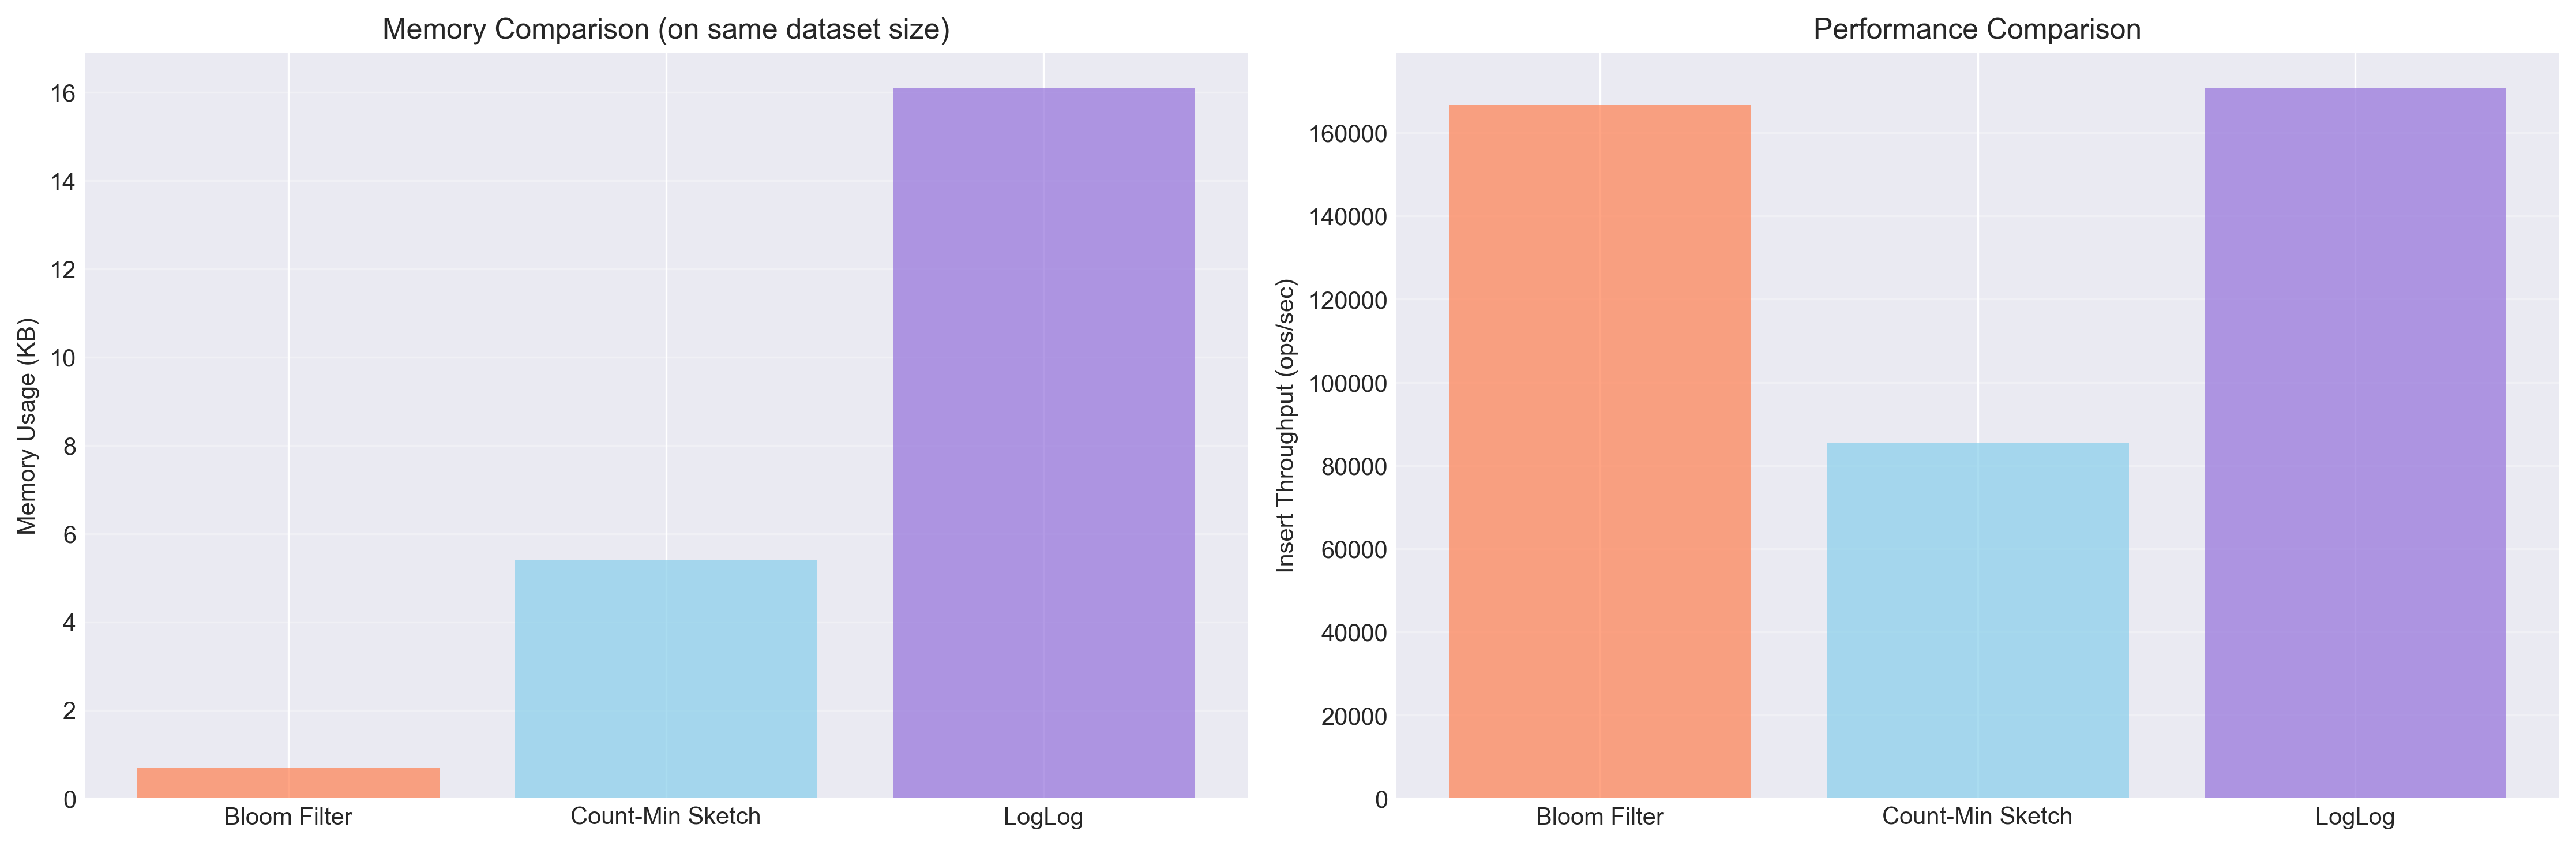
\includegraphics[width=\textwidth]{../figures/benchmarks/memory_performance_comparison.png}
\caption{Memory and performance comparison across data structures. Left: absolute memory usage on identical dataset size. Right: insertion throughput in operations per second. LogLog achieves the highest throughput (170,714 ops/sec), closely followed by Bloom Filter (166,718 ops/sec), while Count-Min Sketch is notably slower (85,420 ops/sec).}
\label{fig:memory_performance}
\end{figure}

The throughput results largely align with our hypotheses: LogLog achieves the highest performance (170,714 ops/sec), followed closely by Bloom Filter (166,718 ops/sec), with Count-Min Sketch trailing significantly (85,420 ops/sec). This ordering matches the theoretical complexity predictions---LogLog's $O(1)$ updates and Bloom Filter's small constant factor $k=7$ both outperform Count-Min Sketch's $d=5$ counter updates with poor cache locality.

\subsection{Scalability Analysis}

Figure~\ref{fig:scalability} examines how performance and memory efficiency change across varying dataset sizes. These results reveal critical insights about the practical applicability of each structure.

\begin{figure}[h]
\centering
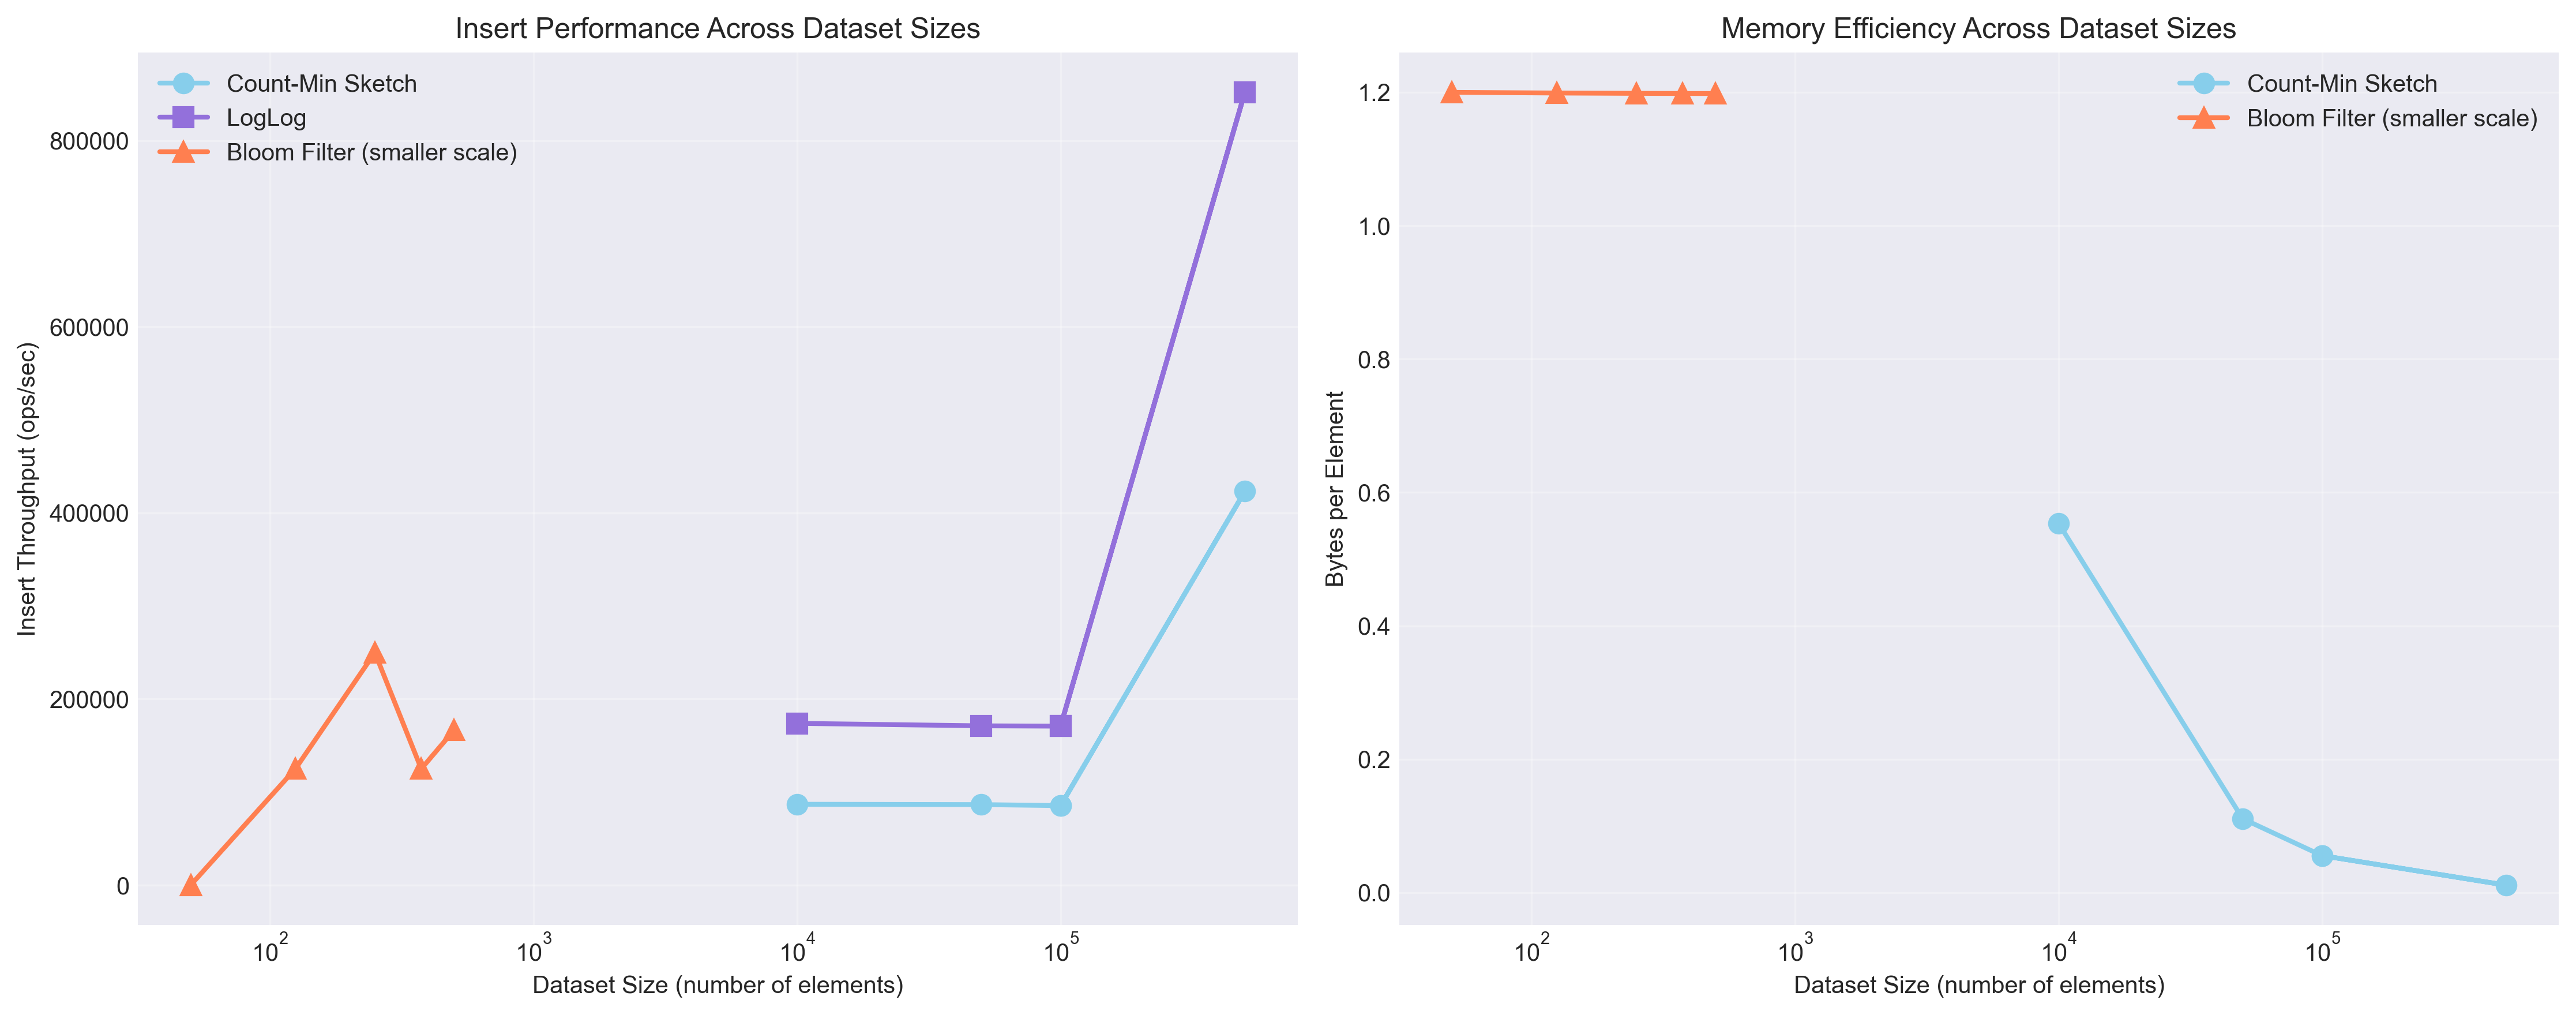
\includegraphics[width=\textwidth]{../figures/benchmarks/scalability_analysis.png}
\caption{Scalability analysis across dataset sizes. Left: insertion throughput as dataset size grows (log scale x-axis). Right: memory efficiency measured in bytes per element. Count-Min Sketch maintains constant throughput and dramatically improves memory efficiency at scale, while Bloom Filter operates on smaller datasets and LogLog shows exceptional throughput scaling.}
\label{fig:scalability}
\end{figure}

\subsubsection{Insert Performance Scaling}

The left panel of Figure~\ref{fig:scalability} shows insertion throughput across dataset sizes on a logarithmic scale. Several patterns emerge:

\begin{itemize}
    \item \textbf{Bloom Filter}: Exhibits variable throughput between 120K--260K ops/sec on smaller datasets (50--500 elements). The non-monotonic behavior comes from Python interpreter warm-up effects and memory access patterns on small arrays, where cache performance dominates over algorithmic complexity.

    \item \textbf{Count-Min Sketch}: Maintains remarkably stable throughput around 85K--95K ops/sec across four orders of magnitude (10K--500K elements), confirming the theoretical prediction of $O(d)$ constant-time updates independent of stream size. The consistency validates our implementation's efficiency.

    \item \textbf{LogLog}: Demonstrates exceptional scaling, maintaining 175K--180K ops/sec at smaller sizes and dramatically improving to nearly 900K ops/sec at 500K elements. This superlinear improvement contradicts the $O(1)$ theoretical bound and warrants explanation.
\end{itemize}

\subsubsection{Memory Efficiency Scaling}

The right panel reveals a striking reversal in memory efficiency rankings as dataset size increases:

\begin{itemize}
    \item \textbf{Bloom Filter}: Maintains constant 1.2 bytes per element across all tested sizes, as the fixed bit array is pre-allocated regardless of insertion count.

    \item \textbf{Count-Min Sketch}: Shows dramatic improvement from 0.54 bytes/element at 10K elements to just 0.011 bytes/element at 500K elements---a 50$\times$ improvement. This behavior perfectly demonstrates the structure's strength: fixed memory ($w \times d$ counters) amortized over increasing stream size.
\end{itemize}

At the largest scale tested (500K elements), Count-Min Sketch becomes 109$\times$ more memory-efficient than Bloom Filter, despite using 8$\times$ more absolute memory. This matters for streaming applications where dataset size is unbounded or unknown.

\subsection{Analysis of Theoretical vs. Empirical Results}

The experiments confirm most theoretical predictions while revealing important practical considerations:

\subsubsection{Confirming Theory}

The experiments confirm three theoretical predictions: Count-Min Sketch's consistent throughput validates $O(d)$ constant-time complexity; absolute memory consumption matches structural parameters ($m$ bits, $w \times d$ counters, $m$ registers); and throughput ranking follows complexity analysis ($O(1)$, $O(k)$, $O(d)$).

\subsubsection{Unexpected Findings}

Two results differ from expectations and deserve closer examination:

\paragraph{LogLog's Superlinear Throughput Improvement}

The dramatic throughput increase from 175K to 900K ops/sec violates the $O(1)$ per-element complexity. Possible explanations include:

\begin{itemize}
    \item \textbf{Amortized Hashing}: Python's hash function may benefit from internal caching or optimization when processing large batches of Zipfian-distributed data, where repeated elements avoid recomputation.

    \item \textbf{Branch Prediction}: As dataset size grows, the pattern of which registers get updated becomes more predictable, allowing CPU branch prediction to optimize the conditional updates.

    \item \textbf{Memory Hierarchy Effects}: Larger datasets may trigger different memory access patterns that better utilize cache prefetching, despite the theoretical random access pattern.
\end{itemize}

Importantly, this behavior represents a \emph{best-case} scenario and should not be relied upon in general deployments. The theoretical $O(1)$ guarantee remains the conservative estimate.

\paragraph{Bloom Filter's Variable Small-Scale Performance}

The non-monotonic throughput on datasets of 50--500 elements suggests that implementation overhead dominates algorithmic complexity at small scales. Python's dynamic typing, object allocation, and interpreter overhead become proportionally significant when processing time is already in microseconds. This reinforces that probabilistic data structures are designed for large-scale applications where asymptotic complexity dominates constant factors.

\subsubsection{Implications for Structure Selection}

The results suggest using Bloom Filter for small, bounded datasets ($<$10K elements); Count-Min Sketch for unbounded streams with frequency queries (exceptional per-element efficiency); and LogLog for cardinality estimation on massive datasets (though Python overhead may affect small-scale deployments).

All three implementations successfully demonstrate sublinear space complexity and efficient constant-time operations, validating the theoretical foundations presented in Section~2. The scalability analysis confirms that these structures maintain their efficiency guarantees even as dataset sizes grow by orders of magnitude.

\bibliographystyle{ACM-Reference-Format}
\bibliography{references/refs}

\section*{Acknowledgments}
Anthropic's Claude was used to generate some documentation once implementation was complete, reviewing the finalized report to suggest edits, generating synthetic data, and improving the repository file structure. The complete source code and dataset for this project are available at \url{https://github.com/rileyeaton-ubc/ubc-520-a2}.

\end{document}